\renewcommand{\theequation}{\theenumi}
\renewcommand{\thefigure}{\theenumi}
\renewcommand{\thetable}{\theenumi}
\begin{enumerate}[label=\thesection.\arabic*.,ref=\thesection.\theenumi]
\numberwithin{equation}{enumi}
\numberwithin{figure}{enumi}
\numberwithin{table}{enumi}

\item A continuous random variable X has a probability density function $f(x) = e^{-x}, 0<x<\infty$. Then $P(X>1)$ is
\begin{enumerate}
\begin{multicols}{4}
\setlength\itemsep{2em}

\item $0.368$
\item $0.5$
\item $0.632$
\item $1.0$

\end{multicols}
\end{enumerate}
%
\solution
We know that,
\begin{align}
\int_{-\infty}^{\infty}{f_x(x)}\,dx = 1.\\
\int_{-\infty}^{0}{f_x(x)}\,dx +\int_{0}^{\infty}{f_x(x)}\,dx = 1\label{ee2016-33:eq_(1)}\\
\int_{-\infty}^{0}{ae^{4x}}\,dx +\int_{0}^{\infty}{\frac{3}{2}e^{-3x}}\,dx = 1\label{ee2016-33:eq_(2)}
\end{align}
The expression \eqref{ee2016-33:eq_(2)} was written from \eqref{ee2016-33:eq_(1)} since,
\begin{align*}
  u(x) = 
  \begin{cases}
  1, & \text{for } x \geq 0\\
  0, & \text{otherwise } 
  \end{cases}
\end{align*}

Simplifying \eqref{ee2016-33:eq_(2)} we have:
\begin{align}
\int_{-\infty}^{0}{ae^{4x}}\,dx +\int_{0}^{\infty}{\frac{3}{2}e^{-3x}}\,dx = 1\nonumber\\
\implies a\left[\frac{e^{4x}}{4}\right]_{-\infty}^{0} +    \frac{3}{2}\left[\frac{e^{-3x}}{-3}\right]_0^{\infty} = 1\\
\implies a\left[\frac{1}{4}-0\right] - \frac{1}{2}\left[0-1\right] = 1\\
\implies \frac{a}{4} + \frac{1}{2} =1 \implies a = 2
\end{align}
Therefore,
\begin{align}
 f_x(x) = 
  \begin{cases}
  \frac{3}{2}e^{-3x}, & \text{for } x \geq 0\\
  2e^{4x}, & \text{for } x < 0
  \end{cases}
\end{align}

The plot for PDF of $X$ can be observed at figure \ref{ee2016-33:fig:The PDF of X}
\begin{figure}[!ht]
       \centering
    \includegraphics[width=.9\columnwidth] {solutions/ee/2016/33/Assignment_2_Fig_2.png}
    \caption{The PDF of X}
    \label{ee2016-33:fig:The PDF of X}
\end{figure}

The CDF of X is defined as follows:
\begin{align}
    F_X(x)= \pr{X\leq x}
\end{align}
Now for $x<0$,
\begin{align}
\pr{X\leq x} &= \int_{-\infty}^{x}{f_x(x)}\,dx\\
&= \int_{-\infty}^{x}{2e^{4x}}\,dx\\
&= 2\left[\frac{e^{4x}}{4}\right]_{-\infty}^{x}\\
&= 2\left[\frac{e^{4x}}{4}-0\right]\\
&= \frac{e^{4x}}{2}
\end{align}
Similarly for $x\geq0$,
\begin{align}
\pr{X\leq x} &= \int_{-\infty}^{x}{f_x(x)}\,dx\\
&= \int_{-\infty}^{0}{2e^{4x}}\,dx +\int_{0}^{x}{\frac{3}{2}e^{-3x}}\,dx\\
&= 2\left[\frac{e^{4x}}{4}\right]_{-\infty}^{0}+\left[\frac{-e^{-3x}}{2}\right]_{0}^{x}\\
&= 2\left[\frac{1}{4}-0\right]-\frac{1}{2}\left[e^{-3x}-1\right]\\
&= 1-\frac{e^{-3x}}{2}
\end{align}

The CDF of X is as below:
\begin{align}
 F_X(x) = 
  \begin{cases}
  1-\frac{e^{-3x}}{2}, & \text{for } x \geq 0\\
  \frac{e^{4x}}{2}, & \text{for } x < 0
  \end{cases}
\end{align}

The plot for CDF of $X$ can be observed at figure \ref{ee2016-33:fig:The PDF of X}.
\begin{figure}[!ht]
       \centering
    \includegraphics[width=.9\columnwidth] {solutions/ee/2016/33/Assignment_2_Fig_1.png}
    \caption{The CDF of X}
    \label{ee2016-33:fig:The CDF of X}
\end{figure}

\begin{align}
\therefore
\pr{X\leq0} = F_X(0)=\frac{1}{2}
\end{align}




\item A random variable X has probability density function $f(x)$ as given below:\\
\begin{align}
f(x) =
\begin{cases}
a+bx
&  0<x<1
\\      
0
& \text{otherwise}
\end{cases}
\label{a}
\end{align}
\\
If the expected value $E[X]=\dfrac{2}{3}$, then $Pr[X<0.5]$ is..........
\\
\solution

We know that the total probability is one,
\begin{equation}
    \int_{-\infty}^{\infty}{f\brak{x} dx} = 1\label{b}
\end{equation}
Using \eqref{a} in \eqref{b},
\begin{align}
    \int_{0}^{1}{(a+bx)\,dx} = 1\\
    \sbrak{ax+\frac{bx^2}{2}}_0^1=1\\
    \left(a+\frac{b}{2}\right)-0=1\\
    \implies a+\frac{b}{2}=1 \label{c}
\end{align}
We know that expectation value of X,
\begin{align}
    E\brak{X}=\int_{-\infty}^{\infty}xf\brak{x}\,dx\label{d}
\end{align}
%
Using $E\brak{X}=\frac{2}{3}$ and \eqref{a} in \eqref{d}, we get
\begin{align}
     \frac{2}{3}&=\int_{0}^{1}x(a+bx)\,dx\\
     &=\int_{0}^{1} ax+bx^2\,dx\\
     &= \sbrak{\frac{ax^2}{2}+\frac{bx^3}{3}}_0^1\\
     &= \frac{a}{2}+\frac{b}{3}-0\\
     \implies\frac{a}{2}+\frac{b}{3}&=\frac{2}{3}\label{e}
\end{align}
By solving \eqref{c} and \eqref{e}, we get 
\begin{align}
    a\, =\, 0 \,\,and\,\, b\, =\, 2.
\end{align}
Using values of $a$ and $b$ in \eqref{a}, we get
\begin{align}
f\brak{x}
= 
\begin{cases}
2x & 0<x<1
\\
0 & otherwise\label{f}\\
\end{cases}
\end{align}
\begin{figure}[ht]
    \centering
    \includegraphics[width=\columnwidth]{solutions/ec/15/figures/assign2.png}
    \caption{Probability Density Function (PDF) of X}
    \label{Figure_1}
\end{figure}
The graph of PDF of X is \ref{Figure_1}
\par Let $F_X(x)$ be the cumulative distribution function of random variable X.
\begin{align}
    F_X(x)=\int_{-\infty}^x f\brak{x} dx\label{x}
\end{align}
$F_X(x)$ can be obtained from the uniform distribution of a random variable U on (0,1) and let U=$X^2$. 
\begin{align}
    0 < U < 1
\end{align}
As for random variable X also,
\begin{align}
    0 < F_X(x) < 1
\end{align}
This similarity between U and $F_X(x)$ is used to generate the random variable X from U.
\begin{align}
    F_X(x)&= \pr{X<x}\\
    &=\pr{\sqrt{U}<x}\\
    &=\pr{U<x^2}\\
    &=F_U(x^2)\label{y}
\end{align}
From uniform distribution,
\\The graph of Probability Density Function (PDF) of U is \ref{Figure_2}
\begin{figure}[ht]
    \centering
    \includegraphics[width=\columnwidth]{solutions/ec/15/figures/assign2_2.png}
    \caption{Probability Density Function (PDF) of U}
    \label{Figure_2}
\end{figure}
\begin{align}
    F_U(x)=
    \begin{cases}
0 & x\leq0\\
x & 0<x<1
\\
1 & x\geq1\label{z}\\
\end{cases}
\end{align}
\begin{figure}[ht]
    \centering
    \includegraphics[width=\columnwidth]{solutions/ec/15/figures/assign2_1.png}
    \caption{Cumulative Density Function (CDF)}
    \label{Figure_3}
\end{figure}
\\Using \eqref{z} in \eqref{y},
\\Cumulative distribution function (CDF) of random variable X is,
\begin{align}
F_X(x)= \pr{X<x}
= 
\begin{cases}
0 & x\leq0\\
x^2 & 0<x<1
\\
1 & x\geq1\label{g}\\
\end{cases}
\end{align}
The graph of Cumulative distribution function (CDF) of random variable X is \ref{Figure_3}\\
Now we have to find \pr{X<0.5},Using  \eqref{g},
\begin{align}
    \pr{X<0.5} &= (0.5)^2\\
  \implies \pr{X<0.5} &= 0.25
\end{align}



\item Let X be a random variable with a probability density function
\begin{align}
f(x) = 
\begin{cases}
0.2 & \abs{x}\leq1
\\
0.1 & 1\leq\abs{x}\leq4
\\
0 & otherwise
\end{cases}
\label{pdf}
\end{align}

Find $\pr{0.5< X \leq 5}$
\\
\solution
\iffalse
\let\negmedspace\undefined
\let\negthickspace\undefined
\documentclass[article]{IEEEtran}
       \def\inputGnumericTable{}                                 %%
\usepackage{cite}
\usepackage{amsmath,amssymb,amsfonts,amsthm}
\usepackage{algorithmic}
\usepackage{graphicx}
\usepackage{textcomp}
\usepackage{xcolor}
\usepackage{txfonts}
\usepackage{listings}
\usepackage{enumitem}
\usepackage{mathtools}
\usepackage{gensymb}
\usepackage[breaklinks=true]{hyperref}
\usepackage{tkz-euclide} % loads  TikZ and tkz-base
\usepackage{listings}
\renewcommand{\theenumi}{\Alph{enumi}}
%
%\usepackage{setspace}
%\usepackage{gensymb}
%\doublespacing
%\singlespacing

%\usepackage{graphicx}
%\usepackage{amssymb}
%\usepackage{relsize}
%\usepackage[cmex10]{amsmath}
%\usepackage{amsthm}
%\interdisplaylinepenalty=2500
%\savesymbol{iint}
%\usepackage{txfonts}
%\restoresymbol{TXF}{iint}
%\usepackage{wasysym}
%\usepackage{amsthm}
%\usepackage{iithtlc}
%\usepackage{mathrsfs}
%\usepackage{txfonts}
%\usepackage{stfloats}
%\usepackage{bm}
%\usepackage{cite}
%\usepackage{cases}
%\usepackage{subfig}
%\usepackage{xtab}
%\usepackage{longtable}
%\usepackage{multirow}
%\usepackage{algorithm}
%\usepackage{algpseudocode}
%\usepackage{enumitem}
%\usepackage{mathtools}
%\usepackage{tikz}
%\usepackage{circuitikz}
%\usepackage{verbatim}
%\usepackage{tfrupee}
%\usepackage{stmaryrd}
%\usetkzobj{all}
    \usepackage{color}                                            %%
    \usepackage{array}                                            %%
    \usepackage{longtable}                                        %%
    \usepackage{calc}                                             %%
    \usepackage{multirow}                                         %%
    \usepackage{hhline}                                           %%
    \usepackage{ifthen}                                           %%
 %optionally (for landscape tables embedded in another document): %%
    \usepackage{lscape}     
%\usepackage{multicol}
%\usepackage{chngcntr}
%\usepackage{enumerate}

%\usepackage{wasysym}
%\documentclass[conference]{IEEEtran}
%\IEEEoverridecommandlockouts
% The preceding line is only needed to identify funding in the first footnote. If that is unneeded, please comment it out.

\newtheorem{theorem}{Theorem}[section]
\newtheorem{problem}{Problem}
\newtheorem{proposition}{Proposition}[section]
\newtheorem{lemma}{Lemma}[section]
\newtheorem{corollary}[theorem]{Corollary}
\newtheorem{example}{Example}[section]
\newtheorem{definition}[problem]{Definition}
%\newtheorem{thm}{Theorem}[section] 
%\newtheorem{defn}[thm]{Definition}
%\newtheorem{algorithm}{Algorithm}[section]
%\newtheorem{cor}{Corollary}
\newcommand{\BEQA}{\begin{eqnarray}}
\newcommand{\EEQA}{\end{eqnarray}}
\newcommand{\define}{\stackrel{\triangle}{=}}
\theoremstyle{remark}
\newtheorem{rem}{Remark}

\begin{document}
\providecommand{\pr}[1]{\ensuremath{\Pr\left(#1\right)}}
\providecommand{\prt}[2]{\ensuremath{p_{#1}^{\left(#2\right)} }}        % own macro for this question
\providecommand{\qfunc}[1]{\ensuremath{Q\left(#1\right)}}
\providecommand{\sbrak}[1]{\ensuremath{{}\left[#1\right]}}
\providecommand{\lsbrak}[1]{\ensuremath{{}\left[#1\right.}}
\providecommand{\rsbrak}[1]{\ensuremath{{}\left.#1\right]}}
\providecommand{\brak}[1]{\ensuremath{\left(#1\right)}}
\providecommand{\lbrak}[1]{\ensuremath{\left(#1\right.}}
\providecommand{\rbrak}[1]{\ensuremath{\left.#1\right)}}
\providecommand{\cbrak}[1]{\ensuremath{\left\{#1\right\}}}
\providecommand{\lcbrak}[1]{\ensuremath{\left\{#1\right.}}
\providecommand{\rcbrak}[1]{\ensuremath{\left.#1\right\}}}
\newcommand{\sgn}{\mathop{\mathrm{sgn}}}
\providecommand{\abs}[1]{\left\vert#1\right\vert}
\providecommand{\res}[1]{\Res\displaylimits_{#1}} 
\providecommand{\norm}[1]{\left\lVert#1\right\rVert}
%\providecommand{\norm}[1]{\lVert#1\rVert}
\providecommand{\mtx}[1]{\mathbf{#1}}
\providecommand{\mean}[1]{E\left[ #1 \right]}
\providecommand{\cond}[2]{#1\middle|#2}
\providecommand{\fourier}{\overset{\mathcal{F}}{ \rightleftharpoons}}
\newenvironment{amatrix}[1]{%
  \left(\begin{array}{@{}*{#1}{c}|c@{}}
}{%
  \end{array}\right)
}
%\providecommand{\hilbert}{\overset{\mathcal{H}}{ \rightleftharpoons}}
%\providecommand{\system}{\overset{\mathcal{H}}{ \longleftrightarrow}}
	%\newcommand{\solution}[2]{\textbf{Solution:}{#1}}
\newcommand{\solution}{\noindent \textbf{Solution: }}
\newcommand{\cosec}{\,\text{cosec}\,}
\providecommand{\dec}[2]{\ensuremath{\overset{#1}{\underset{#2}{\gtrless}}}}
\newcommand{\myvec}[1]{\ensuremath{\begin{pmatrix}#1\end{pmatrix}}}
\newcommand{\mydet}[1]{\ensuremath{\begin{vmatrix}#1\end{vmatrix}}}
\newcommand{\myaugvec}[2]{\ensuremath{\begin{amatrix}{#1}#2\end{amatrix}}}
\providecommand{\rank}{\text{rank}}
\providecommand{\pr}[1]{\ensuremath{\Pr\left(#1\right)}}
\providecommand{\qfunc}[1]{\ensuremath{Q\left(#1\right)}}
	\newcommand*{\permcomb}[4][0mu]{{{}^{#3}\mkern#1#2_{#4}}}
\newcommand*{\perm}[1][-3mu]{\permcomb[#1]{P}}
\newcommand*{\comb}[1][-1mu]{\permcomb[#1]{C}}
\providecommand{\qfunc}[1]{\ensuremath{Q\left(#1\right)}}
\providecommand{\gauss}[2]{\mathcal{N}\ensuremath{\left(#1,#2\right)}}
\providecommand{\diff}[2]{\ensuremath{\frac{d{#1}}{d{#2}}}}
\providecommand{\myceil}[1]{\left \lceil #1 \right \rceil }
\newcommand\figref{Fig.~\ref}
\newcommand\tabref{Table~\ref}
\newcommand{\sinc}{\,\text{sinc}\,}
\newcommand{\rect}{\,\text{rect}\,}
%%
%	%\newcommand{\solution}[2]{\textbf{Solution:}{#1}}
%\newcommand{\solution}{\noindent \textbf{Solution: }}
%\newcommand{\cosec}{\,\text{cosec}\,}
%\numberwithin{equation}{section}
%\numberwithin{equation}{subsection}
%\numberwithin{problem}{section}
%\numberwithin{definition}{section}
%\makeatletter
%\@addtoreset{figure}{problem}
%\makeatother

%\let\StandardTheFigure\thefigure
\let\vec\mathbf

\bibliographystyle{IEEEtran}
\title{
%	\logo{
Assignment
%	}
}
\author{ Karthikeya hanu prakash kanithi (EE22BTECH11026)}
\maketitle
\parindent0px
\vspace{3cm}
Question : Suppose that $(X, Y)$ has joint probability mass function
\begin{align}
P(X = 0, Y = 0) &= P(X = 1, Y = 1) = \theta, \\
P(X = 1, Y = 0) &= P(X = 0, Y = 1) = \frac{1}{2} - \theta.
\end{align}
where $0 \le \theta \le \frac{1}{2}$ is an unknown parameter. Consider testing $H_0 : \theta = \frac{1}{4}$ against $H_1 : \theta = \frac{1}{3}$; based on a random sample ${(X_1 , Y_1 ), (X_2 , Y_2 ), \ldots (X_n , Y_n )}$ from the above probability mass function. Let $M$ be the cardinality of the set $\{i: X_i = Y_i , 1 \le i\le n\}$. If $m$ is the observed value of $M$, then which one of the following statements is true?
\begin{enumerate}
\item The likelihood ratio test rejects $H_0$ if $m > c$ for some $c$.
\item The likelihood ratio test rejects $H_0$ if $m < c$ for some $c$.
\item The likelihood ratio test rejects $H_0$ if $c_1 < m < c_2$ for some $c_1$ and $c_2$.
\item The likelihood ratio test rejects $H_0$ if $m < c_1$ or $m > c_2$ for some $c_1$ and $c_2$.
\end{enumerate}
\fi
\solution 
Given that,
\begin{align}
	H_0 : \quad \theta = \theta_0 = \frac{1}{4},\\
	H_1 : \quad \theta = \theta_1 = \frac{1}{3}.
\end{align}
and the pmf is given by 
\begin{align}
	p_{XY}(0,0) &= p_{XY}(1,1) = \theta \\
	p_{XY}(0,1) &= p_{XY}(1,0) = \frac{1}{2} - \theta 
\end{align}
Then for the given random sample of data, 
\begin{align}
    p_{X_i,Y_i}(x,y) &= 
    \begin{cases}
        2\theta &  x=y  \\
        1 - 2\theta & x\ne y
    \end{cases} \\
\end{align}
Then the likelihood of the data under $H_0$ is given by: 
\begin{align}
    L(\theta_0 \mid data) &= \prod_{i=1}^{n} p_{X_i,Y_i}(x,y) \\
    &= \brak{2\theta_0}^m\brak{1 - 2\theta_0}^{n-m}\\
    &= \brak{\frac{1}{2}}^m\brak{\frac{1}{2}}^{n-m}
\end{align}
Then the likelihood of the data under $H_1$ is given by:
\begin{align}
    L(\theta_1 \mid data) &= \prod_{i=1}^{n} p_{X_i,Y_i}(x,y) \\
    &= \brak{2\theta_1}^m\brak{1 - 2\theta_1}^{n-m}\\
    &= \brak{\frac{2}{3}}^m\brak{\frac{1}{3}}^{n-m}
\end{align}
The likelyhood ratio will be 
\begin{align}
    \lambda(data) &= \frac{L(\theta_1 \mid x)}{L(\theta_0 \mid x)} \\
    &= \frac{\brak{\frac{2}{3}}^m\brak{\frac{1}{3}}^{n-m}}{\brak{\frac{1}{2}}^m\brak{\frac{1}{2}}^{n-m}} = \brak{2}^m\brak{\frac{2}{3}}^{n} \label{eq:st/42/1}
\end{align}
Let the critical value be denoted by $c_1$, then the likelihood ratio test rejects $H_0$ if
\begin{align}
    \implies  \lambda(data) &\overset{H_1}{\underset{H_0}{\gtrless}} c_1\\
\end{align}  
From \eqref{eq:st/42/1},
\begin{align}
    \implies  \brak{2}^m\brak{\frac{2}{3}}^{n} &\overset{H_1}{\underset{H_0}{\gtrless}} c_1\\
    \implies  \brak{2}^m &\overset{H_1}{\underset{H_0}{\gtrless}} c_1\brak{\frac{2}{3}}^{n}\\
    \implies  m &\overset{H_1}{\underset{H_0}{\gtrless}} \log_{2}\brak{c_1\brak{\frac{2}{3}}}^{n}\\
    \implies  m &\overset{H_1}{\underset{H_0}{\gtrless}} c \quad \exists \, c \in \mathbb{R} \label{eq:st/42/2}
\end{align}
where, 
\begin{align}
    c = \log_{2}\brak{c_1\brak{\frac{2}{3}}}^{n}
\end{align}
$\therefore$ From \eqref{eq:st/42/2}, Option A is correct and Options B,C,D are incorrect


%
\item Consider two identically distributed zero-mean random variables U and V. Let the cumulative distribution functions of U and 2V be F(\textit{x}) and G(\textit{x}) respectively. Then,for all values of \textit{x}
\begin{enumerate}
\begin{multicols}{2}
\setlength\itemsep{2em}
{\small
\item $
F(x)-G(x)\leqslant0
$
\item $
F(x)-G(x)\geqslant0
$
\item $
(F(x)-G(x))\textit{x}\leqslant0
$
\item $
(F(x)-G(x))\textit{x}\geqslant0
$
}
\end{multicols}
\end{enumerate}
%
\solution
If $X$ is a random variable, the cumulative distribution functions of U and 2V can be written in terms of $X$ as
\begin{align} \label{equation-1}
    F(x)=\pr{X \leq x} 
\end{align}
\begin{align}
    G(x)=\pr{2X \leq x}
\end{align}
Or,
\begin{align} \label{equation-2}
     G(x)=\pr{X \leq x/2}
\end{align}
Using \ref{equation-1} in \ref{equation-2}, we can see that
\begin{align} \label{equation-3}
    G(x)=F(x/2)
\end{align}
So,
\begin{align}
    F(x)-G(x)=F(x)-F(x/2)
\end{align}
As F is Cumulative Distribution Function, it is non-decreasing.\\
That means for $x \geq y$, $F(x) \geq F(y)$.\\ \\
Using this, we can form the following table:
\begin{table}[h!]
    \centering
    \begin{tabular}{|c|c|c|}
        \hline
        Case & $F(x)-F(x/2)$ & $(F(x)-F(x/2))x$ \\
        \hline
        $x \geq 0$ & $\geq 0$ & $\geq 0$ \\
        \hline
        $x \leq 0$ & $\leq 0$ & $\geq 0$ \\
        \hline
    \end{tabular}
    \caption{}
    \label{table-1}
\end{table}\\
From the table we can see that for any value of $x$,
\begin{align}
    (F(x)-F(x/2))x \geq 0
\end{align}
Or, using \ref{equation-3},
\begin{align}
    (F(x)-G(x))x \geq x
\end{align}
%
\item A probability density function is of the form\\
{\centering $p(\textit{x}) = Ke^{-\alpha |x|}, \textit{x}\in(-\infty,\infty)$\\}
The value of K is 

\begin{enumerate}
\begin{multicols}{4}
\setlength\itemsep{2em}

\item 0.5
\item 1
\item $0.5\alpha$
\item $\alpha$

\end{multicols}
\end{enumerate}


\item The probability density function (PDF) of a random variable X is as shown in Fig. \ref{fig:2}.
\begin{figure}[!h]
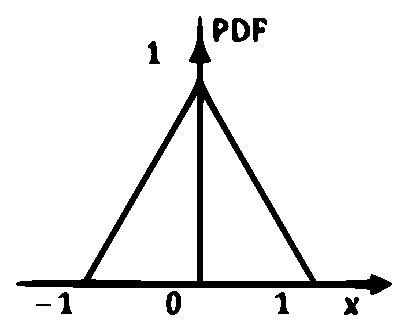
\includegraphics[width=\columnwidth]{./figs/figure2.eps}
\caption{}
\label{fig:2}
\end{figure}

The corresponding cumulative distribution function (CDF) has the form\\

\begin{enumerate}
\begin{multicols}{2}
\setlength\itemsep{4em}

\item Fig. \ref{fig:3}

%\includegraphics{figure3.eps}
\item Fig. \ref{fig:4}

%\includegraphics{figure4.eps}
\item Fig. \ref{fig:5}

% \includegraphics{figure5.eps}
\item Fig. \ref{fig:6}


%\includegraphics{figure6.eps}

\end{multicols}
\end{enumerate}
\begin{figure}[!h]
\includegraphics[width=\columnwidth]{./figs/figure3.eps}
\caption{}
\label{fig:3}
\end{figure}
\begin{figure}[!h]
\includegraphics[width=\columnwidth]{./figs/figure4.eps}
\caption{}
\label{fig:4}
\end{figure}
\begin{figure}[!h]
\includegraphics[width=\columnwidth]{./figs/figure5.eps}
\caption{}
\label{fig:5}
\end{figure}

\begin{figure}[!h]
\includegraphics[width=\columnwidth]{./figs/figure6.eps}
\caption{}
\label{fig:6}
\end{figure}

\item The distribution function $f_x(x)$ of a random variable X is shown in Fig. \ref{fig:12}. The probability that X=1 is
%
\begin{figure}[!h]
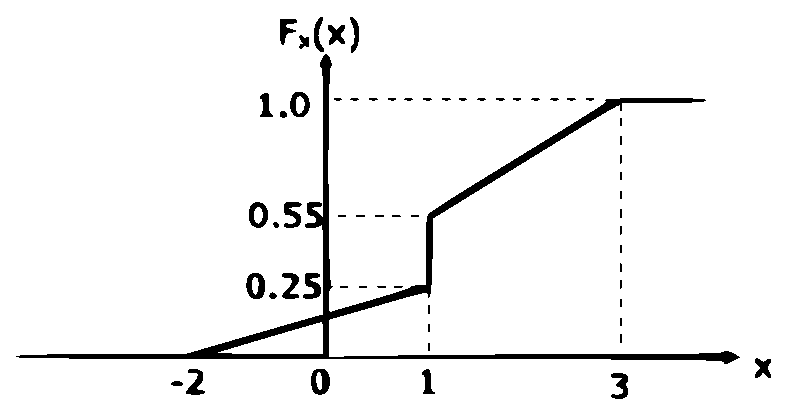
\includegraphics[width=\columnwidth]{./figs/figure12.eps}
\caption{}
\label{fig:12}
\end{figure}


\begin{enumerate}
\begin{multicols}{2}
\setlength\itemsep{1em}

\item Zero
\item 0.25
\item 0.55
\item 0.30

\end{multicols}
\end{enumerate}
%
\item Let the probability density function of a random variable $X$ be 
\begin{center}
$ 
f(x)=
\begin{cases}
x & 0\leq\ x< \frac{1}{2}\\
c(2x-1)^2 &  \frac{1}{2}<x\leq\ 1\\
0 & \text{otherwise}.
\end{cases}
$\\ 
\end{center}


Then,the value of $c$ is equal to \underline{\hspace{3cm}}
\\
\solution
Given X and Y be two continuous random variables with the joint probability density function
\begin{align}
    f\left(x,y\right)=\begin{cases}
    2 \quad  0<x+y<1 ,x>0 ,y>0\\
    0 \quad  \textrm{elsewhere}\\
    \end{cases}
\end{align}
% \begin{figure}[h]
%     \centering
%     \includegraphics[scale=0.2]{f(x,y)_graph.png}
%     \caption{$f\left(x,y\right)$}
%     \label{ec/75/fig:f(x,y)}
% \end{figure}

we know that
\begin{align}
    P\left(\left(x,y\right)\in A\right)=\int \int _{A}f\left(x,y\right) dx dy \quad  A \in \mathbb{R}^2
\end{align}
from given information\\
for positive $x$ and $y$
\begin{align}
    0<x+y<\dfrac{1}{2}  \Rightarrow 0<x<\dfrac{1}{2}-y
\end{align}
so using eq(0.0.3)
\begin{align}
    P\left(x+y < \dfrac{1}{2}\right)=\int_{0}^{\frac{1}{2}} \int _{0}^{\frac{1}{2}-y}f(x,y) dx dy\\
    =\int_{0}^{\frac{1}{2}} \int _{0}^{\frac{1}{2}-y} 2 \quad dx dy
    =\int_{0}^{\frac{1}{2}} \left(  2 x \quad \big|_{0}^{\frac{1}{2}-y} \right)  dy\\
    =\int_{0}^{\frac{1}{2}}   2 \left(\frac{1}{2}-y\right) \quad    dy
    =2\left( \frac{1}{2} y - \frac{y^2}{2}  \right) \big|_{0}^{\frac{1}{2}}\\
    = \left( \frac{1}{2} - \frac{1}{4}\right) = \frac{1}{4} 
\end{align}
Therefore 
\begin{align}
    P\left(X+Y<\dfrac{1}{2}\right)=\dfrac{1}{4}
\end{align}
\begin{align}
\intertext{volume under the graph which contains the region} X+Y<\dfrac{1}{2} \quad \text{gives us} \quad P\left(X+Y<\dfrac{1}{2}\right) \\
 P\left(X+Y<\dfrac{1}{2}\right)= \text{Area of the base . height}
 \end{align}
 
Area of the base triangle is 
\begin{align}
 \dfrac{1}{2}.\textit{height}.\textit{base} =\dfrac{1}{2}.\dfrac{1}{2}.\dfrac{1}{2}
 \end{align}
 \begin{align}
\text{volume = Area . height}=\dfrac{1}{8}. 2= \dfrac{1}{4}
\end{align}
%The volume under the graph which contains the region $X+Y<\dfrac{1}{2}$ %gives us $P\left(x+y<\dfrac{1}{2}\right)$\\
%$P\left(x+y<\dfrac{1}{2}\right)=$ Area of the base . height\\
%Area of the base triangle is $\dfrac{1}{2}.\textit{height}.\textit{base}$%$= \dfrac{1}{2}.\dfrac{1}{2}.\dfrac{1}{2}$\\
%volume = Area . height $= \dfrac{1}{8}. 2= \dfrac{1}{4}$

\begin{figure}[h]
    \centering
    %\columnwidth
    \includegraphics[width=\columnwidth]{solutions/ec/75/P(x+y_2)_graph.png}
    \caption{$P\left(x+y<\dfrac{1}{2}\right)$}
    \label{ec/75/fig:p(x+y<1/2)}
\end{figure}




\item Let $X$ be a random variable with the following cumulative distribution function: 

\begin{center}
$ 
F(x)=
\begin{cases}
0 & x<0 \\
x^2 & 0\leq\ x <\frac{1}{2}\\
\frac{3}{4} & \frac{1}{2}\leq\ x<1\\
1 & x\geq\ 1.
\end{cases}
$\\ 

\end{center}
Then $P\brak{\frac{1}{4}<X<1}$ is equal to \underline{\hspace{3cm}}
\\
\solution
\begin{align}
 P ( a \textless x \textless b ) =  F(b) - F(a) \end{align}
We want, 
 \begin{align}
S&= P ( {\dfrac{1}{4}}  \textless  X \textless  1)\\
S&= F(1) - F(\dfrac{1}{4})  \\
S&= \dfrac{3}{4} - \dfrac{1^2}{4^2} \\
S&= \dfrac{11}{16}
\end{align}
Hence, P( ${\frac{1}{4}}$ $ \textless $ X $\textless $ 1) is equal to $\frac{11}{16}$

\begin{figure}[!ht]
\centering
\includegraphics[width=0.5\textwidth]{solutions/ec/54/codes/graph.png}
\label{ec54:fig:graph.png}
\end{figure}






\item Let $X_1$ be an exponential random variable with mean 1 and $X_2$ a gamma random variable with mean 2 and variance 2. If $X_1$ and $X_2$ are independently distributed,then $P(X_1<X_2)$ is equal to \underline{\hspace{3cm}}
\\
\solution
\begin{enumerate}
    \item Given that $X_1$ is an exponential random variable. Let the P.D.F of $X_1$ be
    \begin{align}
    p_{X_1}(x_1)=
        \begin{cases}
        \lambda e^{-\lambda x_1} & x_1 \geq 0\\
        0 & x_1<0
        \end{cases}
    \end{align}
    C.D.F of $x_1$ is :
    \begin{align}
    \begin{split}
        F_{X_1}(x_1)&=\int_{-\infty}^{x_1} p_{X_1}(x_1) dx_1\\
        &=\int_{-\infty}^0 p_{X_1}(x_1) dx_1+\int_{0}^{x_1} p_{X_1}(x_1) dx_1\\
        &=\int_{-\infty}^0 0 \times dx_1+\int_{0}^ {x_1} \lambda e^{-\lambda x_1} dx_1\\
        &=1-e^{-\lambda x_1}\label{ec55:eq:0.0.2}
        \end{split}
    \end{align}
    \begin{align}
    \text{ As mean}=\lambda\\
     \text{ Given that mean}=1\\
     \text{so } \lambda=1 \label{ec55:eq:0.0.5}
    \end{align} 
     
    \item Given that $X_2$ is an gamma random variable.Let the P.D.F of $X_2$ be:
    \begin{align}
        p_{X_2}(x_2)=
        \begin{cases}
            \frac{a^b x_2^{b-1}e^{-ax_2}}{\Gamma(b)} & x_2\geq 0\\
            0 & x_2<0
        \end{cases}\label{ec55:eq:0.0.6}
    \end{align}
    \begin{align}
       \text{ Since mean}=\frac{b}{a}=2\label{ec55:eq:0.0.7}\\
         \text{Also,variance}=\frac{b}{a^2}=2\label{ec55:eq:0.0.8}
    \end{align}
  From \eqref{ec55:eq:0.0.7} and \eqref{ec55:eq:0.0.8}
  \begin{align}
      b=2,a=1\label{ec55:eq:0.0.9}
  \end{align}
  Since the total probability of $X_2$ is 1 \\
  so,\begin{align}
      \int_{-\infty}^\infty p_{X_2}(x_2) dx_2=1
      \end{align}
      \begin{align}
      \int_{-\infty} ^0 p_{X_2}(x_2)
     dx_2+\int_{0}^\infty p_{X_2}(x_2) dx_2&=1\\
      \int_{-\infty} ^0 0\times dx_2+\int_{0}^\infty \frac{a^b x_2^{b-1}e^{-ax_2}}{\Gamma(b)} dx_2&=1
      \end{align}
      \begin{align}
      \frac{a^b}{\Gamma(b)} \int_{0}^\infty x_2^{b-1}e^{-ax_2} dx_2&=1
      \end{align}
      \begin{align}
          \int_{0}^\infty x_2^{b-1}e^{-ax_2} dx_2&=\frac{\Gamma(b)}{a^b}\label{ec55:eq:0.0.14}
  \end{align}
  now substituting $a+\lambda$ for a in \eqref{ec55:eq:0.0.14} gives 
  \begin{align}
      \int_{0}^\infty x_2^{b-1}e^{-(a+\lambda)x_2} dx_2&=\frac{\Gamma(b)}{(a+\lambda)^b}\label{ec55:eq:0.0.15}
  \end{align}
  Now we have to find $P(X_1<X_2)$\\
  \item Given that $X_1$ and $X_2$ are independent random variables,so
  \begin{align}
     P(X_1<X_2|X_2)=F_{X_1}(X_2)=1-e^{-\lambda X_2}\label{ec55:eq:0.0.16}
  \end{align}
  Now,
\begin{align}
      P(X_1<X_2)&=\int_{0}^\infty F_{X_1}(X_2) \times p_{X_2}(x_2)dx_2
      \end{align}
      from \eqref{ec55:eq:0.0.6},\eqref{ec55:eq:0.0.16}
  \begin{align}
     P(X_1<X_2)=\int_{0}^\infty (1-e^{-\lambda X_2})\times \frac{a^b x_2^{b-1}e^{-ax_2}}{\Gamma(b)} dx_2
     \end{align}
     \begin{align}
     P(X_1<X_2)=\frac{a^b}{\Gamma(b)}\int_{0}^\infty x_2^{b-1}(e^{-ax_2}-e^{-(a+\lambda)x_2})dx_2
  \end{align}
      from \eqref{ec55:eq:0.0.14} and \eqref{ec55:eq:0.0.15}
      \begin{align}
     P(X_1<X_2)&=\frac{a^b}{\Gamma(b)}\brak{\frac{\Gamma(b)}{a^b}-\frac{\Gamma(b)}{(a+\lambda)^b}}
     \end{align}
 \begin{align}
      P(X_1<X_2)=1-\frac{a^b}{(a+\lambda)^b}
 \end{align}
 \begin{align}
     P(X_1<X_2)=1-\brak{\frac{a}{a+\lambda}}^b
 \end{align}
 from \eqref{ec55:eq:0.0.5} and \eqref{ec55:eq:0.0.9}
 \begin{align}
     P(X_1<X_2)&=1-\brak{\frac{1}{1+1}}^2\\
     P(X_1<X_2)&=1-\frac{1}{4}=\frac{3}{4}
 \end{align}
\end{enumerate}

\begin{center}
\centering\underline{\textbf{Common Data for the next two Questions :}}
\end{center}

\item 
Let $X$ and $Y$ be jointly distributed random variables such that the conditional distribution of $Y$, given $X$ =$x$, is uniform on the interval $(x-1,x+1)$. Suppose $E(X)=1$ and $Var(X)=\frac{5}{3}$.
\\
The mean of the random variable $Y$ is 
\begin{enumerate}
\begin{multicols}{2}
\setlength\itemsep{2em}

\item $ \frac{1}{2}$\\
\item $1$\\
\item $ \frac{3}{2}$\\
\item $2$

\end{multicols}
\end{enumerate}
\solution
We know that,
\begin{equation}
    f_{Y|X=x}(y)=\frac{f(x,y)}{f_{X}(x)} \label{ec56:eq:2.0.1}
\end{equation}
Given that $f_{Y|X=x}(y)$ is uniform over the interval (x-1,x+1).
\begin{equation}
    \Rightarrow f_{Y|X=x}(y)=
    \begin{cases}
    \frac{1}{2} & y \in \brak{x-1,x+1}\\
    0 & \text{otherwise}
    \end{cases}\label{ec56:eq:2.0.2}
\end{equation}
Given $E(X)=1$
\begin{equation}
    \Rightarrow \int_{-\infty}^{\infty}x f_{X}(x)dx=1 \label{ec56:eq:2.0.3}
\end{equation}
Now consider $E(Y|X=x)$,
\begin{equation}
    E(Y|X=x)=\int_{-\infty}^{\infty}yf_{Y|X=x}(y)dy
\end{equation}
From \eqref{ec56:eq:2.0.2} it simplifies to,
\begin{multline}
    \Rightarrow E(Y|X=x)=\int_{-\infty}^{x-1}yf_{Y|X=x}(y)dy+\\ \int_{x-1}^{x+1}yf_{Y|X=x}(y)dy+\int_{x+1}^{\infty}yf_{Y|X=x}(y)dy
\end{multline}
\begin{align}
    \Rightarrow E(Y|X=x)&=\int_{x-1}^{x+1}y\brak{\frac{1}{2}}dy\\
    &=x
\end{align}
Now we can write ,\\
\begin{align}
    E(Y)&=\int_{-\infty}^{\infty}E(Y|X=x)f_{X}(x)dx\\
    &=\int_{-\infty}^{\infty}xf_{X}(x)dx\\
    &=E(X)
\end{align}
From \eqref{ec56:eq:2.0.3} we get 
\begin{equation}
    E(Y)=1.
\end{equation}
\item The variance of the random variable $Y$ is 
\\
\begin{enumerate}
\begin{multicols}{2}
\setlength\itemsep{2em}

\item $ \frac{1}{2}$\\
\item $ \frac{2}{3}$\\
\item $1$\\
\item $2$

\end{multicols}
\end{enumerate}
\solution
\input{solutions/ec/57.tex}

\item Let the random variable $X$ have the distribution function: 
\begin{center}
$ 
F(x)=
\begin{cases}
0 &  \ x<0 \\
\frac{x}{2} &  \ 0\leq\ x <1 \\
\frac{3}{5} &  \ 1\leq\ x<2\\
\frac{1}{2}+\frac{x}{8} &  \ 2\leq\ x<3\\
1 &  \ x\geq\ 3.
\end{cases}
$\\ 
\end{center}

Then $P\brak{2 \leq\ X<4}$ is equal to \underline{\hspace{3cm}}
 \\
\solution
Given that, the CDF of the given random variable is
$$
F_X(x)=\begin{cases}
			x/2, & 0<x<\frac{1}{2}\\
            x, & \frac{1}{2}\leq x\leq 1
		 \end{cases}
$$
% \begin{figure}[h]
%     \includegraphics[width = 8cm]{images/Assignment_2.png}
% \end{figure}
that means probability of the random variable being $m$ is
\begin{align}
\Pr(X = m) =F_X(m) -  \lim_{t \to m^-}F_X(t)
\end{align}
Hence the probability value at $ X =\frac{1}{2}$ is
\begin{align}
    \Pr(X = 1/2) &= F_X\brak{\dfrac{1}{2}} -\lim_{t \to \frac{1}{2}^-}F_X(t)\\
    &= \frac{1}{2} - \lim_{x \to \frac{1}{2}^-} \frac{x}{2}\\
    &= \frac{1}{2} - \frac{1}{4}\\
    &= \frac{1}{4} = 0.25
\end{align}

%
\item Let $X$ be a random variable having the distribution function: 
\begin{center}
$ 
F(x)=
\begin{cases}
0 &  \ x<0 \\
\frac{1}{4} &  \ 0\leq\ x <1 \\
\frac{1}{3} &  \ 1\leq\ x<2\\
\frac{1}{2} &  \ 2\leq\ x<\frac{11}{3}\\
1 &  \ x\geq\ \frac{11}{3}.
\end{cases}
$\\ 
\end{center}

Then $E(X)$ is equal to \underline{\hspace{3cm}}
%
\item Let $\Omega= (0,1]$ be the sample space and let $P(\cdot)$ be a probability function defined by 

\begin{center}
$ 
P((0,x])=
\begin{cases}
\frac{x}{2} &  \ 0 \leq\ x< \frac{1}{2} \\
x &  \  \frac{1}{2} \leq\ x \leq\ 1.
\end{cases}
$\\ 
\end{center}

Then $P\brak{\lbrace\frac{1}{2}\rbrace}$ is equal to \underline{\hspace{3cm}}
%
\item Suppose the random variable $U$ has uniform distribution on $[0,1]$ and $X= -2\log U$. The density of $X$ is

\begin{enumerate}

\item $ 
f(x)=
\begin{cases}
e^{-x} &  \ x>0\\
0 & \text{otherwise}.
\end{cases}
$\\ 

\item $ 
f(x)=
\begin{cases}
2e^{-2x} & \ x>0\\
0 & \text{otherwise}.
\end{cases}
$\\ 

\item $ 
f(x)=
\begin{cases}
\frac{1}{2}e^{-\frac{x}{2}} &  \ x>0\\
0 & \text{otherwise}.
\end{cases}
$\\ 

\item $ 
f(x)=
\begin{cases}
\frac{1}{2} &  \ x \in [0,2]\\
0 & \text{otherwise}.
\end{cases}
$\\ 



\end{enumerate}

\item Suppose $X$ is a real-valued random variable.Which of the following values \textbf{CANNOT} be attained by $E[X]$ and $E[X^2]$, respectively?


\begin{enumerate}
\begin{multicols}{2}
\setlength\itemsep{2em}

\item $
0 \ and \ 1
$
\item $
2  \ and \ 3
$
\item $
\frac{1}{2} \ and \ \frac{1}{3}
$
\item $
2 \ and \ 5
$

\end{multicols}
\end{enumerate}
\solution
\input{solutions/ec/63.tex}

\item Let $\Omega = (0,1]$ be the sample space and let $P(.)$ be a probability function defined by \\
$
P((0,x])=
\begin{cases}
\frac{x}{2} 
&  0 \leqslant x < \frac{1}{2} \\
x &  \frac{1}{2} \leqslant x \leqslant 1
\end{cases}
$ \\
Then $P \bigg ( \{ \frac{1}{2} \} \bigg )$ is equal to.......

\item Let X be a random variable with the following cumulative distribution function: \\

$
F(x)= 
\begin{cases}
0 & x<0 \\
x^2 & 0 \leqslant x < \frac{1}{2} \\
\frac{3}{4} & \frac{1}{2} \leqslant x < 1 \\
1 & x \geqslant 1
\end{cases}
$ \\

Then $P({\frac{1}{4}}<x<1)$ is equal to........
\\
\solution
\input{solutions/ec/73/Assignment-2.tex}

\item Let $X_1$ be an exponential random variable with mean 1 and $X_2$ a gamma random variable with mean 2 and variance 2. If $X_1$ and $X_2$ are independently distributed, then $P(X_1<X_2)$ is equal to.....

\item Suppose the random variable U has uniform distribution on $[0,1]$ and $X= -2 \log U$. The density of X is \\

\begin{enumerate}
\setlength\itemsep{2em}

\item $
f(x)=
\begin{cases}
e^{-x} &  x>0\\
0 & \text{otherwise}
\end{cases}
$

\item $
f(x)=
\begin{cases}
2e^{-2x} &  x>0 \\
0 & \text{otherwise}
\end{cases}
$

\item $
f(x)=
\begin{cases}
\dfrac{1}{2}e^-{\frac{x}{2}} &  x>0 \\
0 & \text{otherwise}
\end{cases}
$

\item $
f(x)=
\begin{cases}
\dfrac{1}{2} &  x \in [0,2] \\
0 & \text{otherwise}
\end{cases}
$

\end{enumerate}
\solution
$U$ - uniformly distributed random variable on $\in$ [0,1]. 
Probability density function of $U$ is: 
\begin{align}
    f_U(u) =
    \begin{cases}
     1  & x \in  [0,1] \\
    0 & \text{otherwise} 
    \end{cases}
\end{align}
 $X$ is given by :
\begin{align}
  X = -2 \ln(U) \\
\implies    0 \leq X \leq \infty
\end{align}
CDF of  $X$ is defined as 
\begin{align}
    F_X(x) &= \pr{X \le x} \\
           &= \pr{-2 \ln(U)\le x} \\
           &= \pr{\ln(U) \ge( -x) /2}\\
           &= \pr {U \ge \exp(-x/2)}\\
           &= 1 - \pr{U \le exp(-x/2)}\\
           &= 1 - exp(-x/2) 
\end{align}
where x $\in$ [0,$\infty$] \\
PDF of $X$ : 
\begin{align}
    f_X(x) & = \frac{d (F_X (x)) }{dx} \\
           & = \frac{1}{2}  exp((-x)/2)
\end{align}
 we have     
\begin{align}
    0 \leq X \leq \infty
\end{align}
\begin{align}
    f_X(x) =
    \begin{cases}
    \frac{1}{2}  exp(\frac{-x}{2}) & x > 0 \\
    0 & \text{otherwise}
    \end{cases}
\end{align}
$\therefore$ answer will be option \brak 3


\item Suppose X is a real-valued random variable. Which of the following values CANNOT be attained by $E[X]$ and $E[X^2]$, respectively?

\begin{enumerate}
\begin{multicols}{2}
\setlength\itemsep{2em}

\item 0 and 1
\item 2 and 3
\item $\dfrac{1}{2}$ and $\dfrac{1}{3}$
\item 2 and 5
\end{multicols}
\end{enumerate}
\solution
%
Since events $E_1$ and $E_2$ are independent, 
\begin{align}
    \pr{E_1E_2}&=\pr{E_1}\times\pr{E_2} \nonumber\\\nonumber\\
    \pr{E_2|E_1}&=\frac{\pr{E_1E_2}}{\pr{E_1}} = \pr{E_2} \nonumber\\ \nonumber\\
     \therefore \pr{E_2} &= \frac{1}{2}
\end{align}
\\[1000pt]
From the given information we get,\\
\begin{table}[h]
\centering
    \begin{tabular}{|c|c|c|}
        \hline
         &0 &1    \\ \hline
        $\pr{X}$ &$\frac{3}{4}$ &$\frac{1}{4}$   \\ \hline
        $\pr{Y}$ &$\frac{1}{2}$ &$\frac{1}{2}$ \\ \hline
    \end{tabular}
\caption{Probability of $X \in \{0,1\}$ and $Y \in \{0,1\}$}
\label{ma2003-80:table=1}
\end{table}
%
$F_X(x)=
\begin{cases}
1, &x\geq1\\
\frac{3}{4}, & 0\leq x \leq1\\
0, &x<0
\end{cases}$
$F_Y(y)=
\begin{cases}
1, &y\geq1\\
\frac{1}{2}, & 0\leq y \leq1\\
0, &y<0
\end{cases}$
\\
\begin{enumerate}[label=(\arabic*)]
    \item $X$ is not uniformly distributed on the set $\{0,1\}$ as it is not continuous in $\{0,1\}$ (both $X$ and $Y$ are Bernoulli Distributions).\\
    $\therefore$ Statement $\alpha$ is incorrect.\label{ma2003-80:a}\\ 
    \item Since $F_X(x)\neq F_Y(y)$, $X$ and $Y$ are not identically distributed.\\
    $\therefore$ Statement $\beta$ is incorrect.\label{ma2003-80:b}\\
    \item $\pr{X^2+Y^2=1}$\label{ma2003-80:c}
    \begin{align}
        &=\pr{X=0,Y=1}+\pr{X=1,Y=0}\nonumber\\
        &= \frac{1}{2}
    \end{align}
    $\therefore$ Statement $\gamma$ is correct.\\
    \item $\pr{XY=X^2Y^2}$\label{ma2003-80:d}
    \begin{align}
        &=\sum_{i=0}^1\sum_{j=0}^1\pr{X=i,Y=j}\nonumber\\
        &= 1
    \end{align}
    $\therefore$ Statement $\delta$ is correct.\\
\end{enumerate}
\begin{enumerate}[label=(\alph*)]
    \item This option is incorrect as statement $\alpha$ is incorrect \ref{ma2003-80:a} and statement $\beta$ is incorrect \ref{ma2003-80:b}.\\
    \item This option is incorrect as statement $\gamma$ is correct \ref{ma2003-80:c} but statement $\alpha$ is incorrect \ref{ma2003-80:a}.\\
    \item This option is incorrect as statement $\gamma$ is correct \ref{ma2003-80:c} but statement $\beta$ is incorrect \ref{ma2003-80:b}.\\
    \item This option is correct as statement $\gamma$ is correct \ref{ma2003-80:c} and statement $\delta$ is correct \ref{ma2003-80:d}.\\
\end{enumerate}
$\therefore$ Option (d), $(\gamma,\delta)$, is the answer.

\item Probability density function $p(x)$ of a random variable x is as shown below. The value of $\alpha$ is 

\begin{figure}[!h]
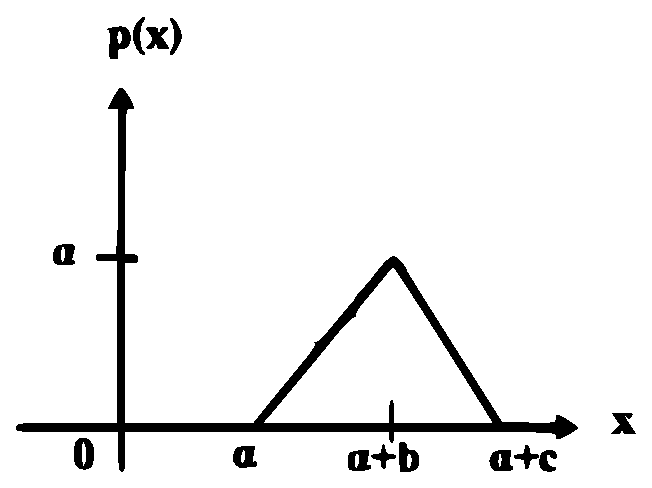
\includegraphics[width=\columnwidth]{./figs/figure13.eps}
\caption{}
\label{fig:13}
\end{figure}


\begin{enumerate}
\begin{multicols}{2}
\setlength\itemsep{2em}

\item $\dfrac{2}{c}$
\item $\dfrac{1}{c}$
\item $\dfrac{2}{(b+c)}$
\item $\dfrac{1}{(b+c)}$

\end{multicols}
\end{enumerate}


%
\item Let the probability density function of random variable,$X$,be given as:\\
\\$f_x(x)$ = $\frac{3}{2}$$e^{-3x}$${u(x)}$ + $a$$e^{4x}$${u(-x)}$\\
\\where u(x) is the unit step function.Then the value of a and Prob\{$X\leq0$\}, respectively,are:\\
\\(A) 2,$\frac{1}{2}$\\
\\(B) 4,$\frac{1}{2}$\\
\\(C) 2,$\frac{1}{4}$\\
\\(D) 4,$\frac{1}{4}$\\
\solution
We know that,
\begin{align}
\int_{-\infty}^{\infty}{f_x(x)}\,dx = 1.\\
\int_{-\infty}^{0}{f_x(x)}\,dx +\int_{0}^{\infty}{f_x(x)}\,dx = 1\label{ee2016-33:eq_(1)}\\
\int_{-\infty}^{0}{ae^{4x}}\,dx +\int_{0}^{\infty}{\frac{3}{2}e^{-3x}}\,dx = 1\label{ee2016-33:eq_(2)}
\end{align}
The expression \eqref{ee2016-33:eq_(2)} was written from \eqref{ee2016-33:eq_(1)} since,
\begin{align*}
  u(x) = 
  \begin{cases}
  1, & \text{for } x \geq 0\\
  0, & \text{otherwise } 
  \end{cases}
\end{align*}

Simplifying \eqref{ee2016-33:eq_(2)} we have:
\begin{align}
\int_{-\infty}^{0}{ae^{4x}}\,dx +\int_{0}^{\infty}{\frac{3}{2}e^{-3x}}\,dx = 1\nonumber\\
\implies a\left[\frac{e^{4x}}{4}\right]_{-\infty}^{0} +    \frac{3}{2}\left[\frac{e^{-3x}}{-3}\right]_0^{\infty} = 1\\
\implies a\left[\frac{1}{4}-0\right] - \frac{1}{2}\left[0-1\right] = 1\\
\implies \frac{a}{4} + \frac{1}{2} =1 \implies a = 2
\end{align}
Therefore,
\begin{align}
 f_x(x) = 
  \begin{cases}
  \frac{3}{2}e^{-3x}, & \text{for } x \geq 0\\
  2e^{4x}, & \text{for } x < 0
  \end{cases}
\end{align}

The plot for PDF of $X$ can be observed at figure \ref{ee2016-33:fig:The PDF of X}
\begin{figure}[!ht]
       \centering
    \includegraphics[width=.9\columnwidth] {solutions/ee/2016/33/Assignment_2_Fig_2.png}
    \caption{The PDF of X}
    \label{ee2016-33:fig:The PDF of X}
\end{figure}

The CDF of X is defined as follows:
\begin{align}
    F_X(x)= \pr{X\leq x}
\end{align}
Now for $x<0$,
\begin{align}
\pr{X\leq x} &= \int_{-\infty}^{x}{f_x(x)}\,dx\\
&= \int_{-\infty}^{x}{2e^{4x}}\,dx\\
&= 2\left[\frac{e^{4x}}{4}\right]_{-\infty}^{x}\\
&= 2\left[\frac{e^{4x}}{4}-0\right]\\
&= \frac{e^{4x}}{2}
\end{align}
Similarly for $x\geq0$,
\begin{align}
\pr{X\leq x} &= \int_{-\infty}^{x}{f_x(x)}\,dx\\
&= \int_{-\infty}^{0}{2e^{4x}}\,dx +\int_{0}^{x}{\frac{3}{2}e^{-3x}}\,dx\\
&= 2\left[\frac{e^{4x}}{4}\right]_{-\infty}^{0}+\left[\frac{-e^{-3x}}{2}\right]_{0}^{x}\\
&= 2\left[\frac{1}{4}-0\right]-\frac{1}{2}\left[e^{-3x}-1\right]\\
&= 1-\frac{e^{-3x}}{2}
\end{align}

The CDF of X is as below:
\begin{align}
 F_X(x) = 
  \begin{cases}
  1-\frac{e^{-3x}}{2}, & \text{for } x \geq 0\\
  \frac{e^{4x}}{2}, & \text{for } x < 0
  \end{cases}
\end{align}

The plot for CDF of $X$ can be observed at figure \ref{ee2016-33:fig:The PDF of X}.
\begin{figure}[!ht]
       \centering
    \includegraphics[width=.9\columnwidth] {solutions/ee/2016/33/Assignment_2_Fig_1.png}
    \caption{The CDF of X}
    \label{ee2016-33:fig:The CDF of X}
\end{figure}

\begin{align}
\therefore
\pr{X\leq0} = F_X(0)=\frac{1}{2}
\end{align}




%
\item Suppose $X_i$ for $i = 1, 2, 3$ are independent
and identically distributed random variables
whose probability mass functions are
$\pr{X_i = 0} = \pr{X_i = 1} = \frac{1}{2}$ for $i = 1, 2, 3$.
Define another random variable $Y = X_1 X_2 \oplus X_3$, where $\oplus$ denotes XOR. Then $\pr{Y = 0|X_3 = 0} =$
\\
\solution 

For
\begin{align}
    \because Y = (X_1X_2) \oplus X_3 &= 0\\
    \implies X_1X_2 &= X_3 \label{cs2015-37:all_equal}
\end{align}
\begin{align}
    \pr{Y=0|X_3=0} &= \dfrac{\pr{Y=0,X_3=0}}{\pr{X_3=0}} \label{cs2015-37:eq:0.0.1}\\
    &=\dfrac{\pr{X_1X_2 = X_3, X_3 = 0}}{\pr{X_3=0}}\\
    \pr{X_3 = 0} &= \frac{1}{2} \label{cs2015-37:eq:0.0.2}
\end{align}
if $X_3 = 0$, from \eqref{cs2015-37:all_equal}
\begin{align}
    X_1X_2 &= 0
\end{align}
%The number of possibilities for $X_1X_2=0$
%\begin{align}
%    (X_1,X_2) = \begin{cases}
%(0,0)\\(0,1)\\(1,0)
%\end{cases}
%\end{align}
The random variables are independent of each other:
%\begin{align}
%    \pr{X_i = a, X_j = b} &= \pr{X_i=a} \cdot \pr{X_j=b}\\
%    i \neq j,\quad i,j &\in \{1,2,3\}\\
%    a,b &\in \{0,1\}
%\end{align}
\begin{table}[h!]
    \centering
    \resizebox{\columnwidth}{!}
    {
    \begin{tabular}{|c|c|c|}
    \hline
         $\pr{X_1=0,X_2=0}$& $\pr{X_1=0}\cdot\pr{X_2=0}$&$0.25 $\\ \hline
         
         $\pr{X_1=1,X_2=0}$&$\pr{X_1=1}\cdot\pr{X_2=0}$&$0.25$ \\  \hline
         $\pr{X_1=0,X_2=1}$&$\pr{X_1=0}\cdot\pr{X_2=1}$&$0.25$\\
         \hline
    \end{tabular}
    }
    
    \caption{Probabilities }
    \label{cs2015-37:tab:my_label}
\end{table}
\begin{align}
\nonumber
\pr{X_1X_2=0} &= \pr{X_1=0,X_2=0} \\ \nonumber
    &\quad+ \pr{X_1=0,X_2=1}\\ &\quad+ \pr{X_1=1,X_2=0}\\
    &=\frac{1}{4} +\frac{1}{4} + \frac{1}{4}= \frac{3}{4} 
\end{align}
\begin{align}
    \pr{Y=0,X_3=0} &= \pr{X_1X_2=X_3=0}\\
    &= \pr{X_1X_2=0}\cdot\pr{X_3=0}\\
    &=\frac{3}{4} \cdot \frac{1}{2}\\
    &=\frac{3}{8} \label{cs2015-37:case_A}
\end{align}
Upon substituting \eqref{cs2015-37:case_A} and \eqref{cs2015-37:eq:0.0.2} in \eqref{cs2015-37:eq:0.0.1}
\begin{align}
    \pr{Y=0|X_3=0} = \dfrac{3}{4} = 0.75
\end{align}

%
\item A continuous random variable X has a probability density function 
\begin{align}
 \fn{x} = e^{-x}, \text{where, } 0<x<\infty.
\end{align}
Then \pr{X > 1} is ?
\solution

The total number of black balls are 5\\
Number of black balls initially present + number of black balls added =5\\
So, the number of black balls initially in the urn is 5-3=2\\
Let X be the random variable denoting the number of black balls in the urn. So, by binomial distribution, 
\begin{align}
    \pr{X=1}&=p\\
    \pr{X=k}&= {n\choose k} p^k (1-p)^{n-k}\\ \label{ma2018-11:eq}
    k&=0,1,2,...,n
\end{align}
For the given problem, $n=4$ and $p=0.5$, because there is equal probability for each ball of being white or black.
For having exactly 2 black balls, \\
From \eqref{ma2018-11:eq},
\begin{align}
    \pr{X=2}&= {4 \choose 2} \left(\frac{1}{2}\right)^2\left(\frac{1}{2}\right)^2\\
    &=\frac{6}{16}\\
    &=\frac{3}{8}
\end{align}

%
\item Assume that the duration in minutes of a telephone conversation follows the exponential distribution f(x) = $\frac{1}{5}e^{-\frac{x}{5}}$, x $\ge$ 0. The probability that the conversation will exceed five minutes is...
\begin{enumerate}
\item $\frac{1}{e}$ 
\item 1 - $\frac{1}{e}$ 
\item $\frac{1}{e^2}$ 
\item 1 - $\frac{1}{e^2}$
\end{enumerate}
%
%
\solution

Let X be a Random variable defined,that denotes the duration of a telephonic conversation in minutes.\\
So, X $\in$ [0,$\infty$) \\
Given, f$_X$(x) = $\frac{1}{5}e^{-\frac{x}{5}}$ \\
Let CDF of X be F$_X$(x)
\begin{align*}
F_X(x) &=  \int_{-\infty}^{x}f_X(t) \,dt \\
       &= \int_{-\infty}^{0}f_X(t) \,dt + \int_{0}^{x}f_X(t) \,dt \\
F_X(x) &= \int_{0}^{x}f_X(t) \,dt  \because f_X(x) = 0 \forall x<0  \\
\therefore F_X(x) &= \int_{0}^{x}\frac{1}{5}e^{-\frac{t}{5}} \,dt \\
\tag{1}
\label{in2007-27:CDF}
\implies F_X(x) &= 1 - e^{-\frac{x}{5}}
\end{align*}
\begin{align*}
F_X(x) &= \pr{X \le x} \\
\pr{X > 5} &= 1 - \pr{X \le 5} \\
\implies \pr{X > 5} &= 1 - F_X(5) \\
 &= 1 - (1 - e^{-\frac{5}{5}}) \\
 &= e^{-\frac{5}{5}}  \\
 &= e^{-1} = \frac{1}{e}
\end{align*}

%
\item Suppose $Y$ is distributed uniformly in the open interval (1,6). The probability that the polynomial 3$x^2$+6$xY$+3$Y$+6 has only real roots is (rounded off to 1 decimal place) 
%
\solution
 Given, $Y$ has a uniform distribution in the interval (1,6).  
This implies, the probability density function of $Y$,
\begin{align}
f\brak{y} 
= 
\begin{cases}
\frac{1}{6-1} = \frac{1}{5}           & (1<y<6) \\
0           & $otherwise$ 
\end{cases}
\end{align}
 
From this, cumulative distribution function of $Y$, 
\begin{align}
F_Y\brak{y} 
= 
\begin{cases}
\frac{y-1}{5}           & (1<y<6) \\
0           & y \leq 1 \\
1           & y \geq 6 \\
\end{cases}
\end{align}
  Given polynomial: 3$x^2$+(6$Y)x$+(3$Y$+6)  Comparing it with the form: a$x^2$+b$x$+c 

Here, a=3; b=$6Y$; c=$3Y+6$
 Condition for real roots,
\begin{align}
    b^2 - 4ac \geq 0\\
    (6Y)^2 - 4(3)(3Y+6) \geq 0 \\
    Y^2-Y-2 \geq 0\\
 (Y-2)(Y+1) \geq 0
 \end{align}
 \begin{align}
\therefore  Y \leq -1, &  Y \geq 2
\end{align}
Probability that the given polynomial has real roots is,
\begin{align}
   P\brak{Y \leq -1} + P\brak{Y \geq 2} &= F_Y\brak{-1} + 
       1 - F_Y\brak{2^{-}}\\
      &= 0 + 1 - \brak{\frac{2-1}{5}}\\
    &= 0.8
\end{align}

%
\item Let \(X\) be a continuous random variable denoting the temperature measured. The range of temperature is [0,100] degree Celsius and let probability density function of \(X\) be \(f(x)\)=0.01 for 0 \(\leq X \leq\) 100.\newline
The mean of \(X\) is ?\newline
%
\begin{enumerate}[label=(\Alph*)]
    \item \(2.5\)
    \item \(5.0\)
    \item \(25.0\)
    \item \(50.0\)
\end{enumerate}
%
\solution
Given \(X\) is a continuous random variable.
The probability density function of X is \(f(x)\)

\begin{align}
    f(x) = 
	\begin{cases}
	0.01 &  0 \leq x \leq 100\\ ~\\[-1em]
	0 & \text{otherwise}
	\end{cases}
\end{align}
\begin{flushleft}
Mean of the random variable X is \(\mu\)
\end{flushleft}
\begin{align}
    \mu &= \int\limits_{-\infty}^{\infty} x\,f(x)\,\mathrm{d}x =\displaystyle\int\limits_{0}^{100} x\,(0.01)\,\mathrm{d}x\\\nonumber\\
    &=(0.01)\displaystyle\int\limits_{0}^{100} x\,\mathrm{d}x = (0.01)\;\;\frac{x^2}{2}\bigg\vert_0^{100}\\\nonumber\\
    &=50.0 \text{  degree Celsius}\\\nonumber
\end{align}


%
\item The PDF of a Gaussian random variable X is given by 
P$_{X}(x) = \dfrac{1}{3\sqrt{2\pi}}e^{\dfrac{-(x-4)^{2}}{18}}$.The probability of the event { X = 4} is\\
\begin{enumerate}
    \item  $\dfrac{1}{2}$\\
    \item  $\dfrac{1}{3\sqrt{2\pi}}$\\
    \item  0\\
    \item  $\dfrac{1}{4}$\\
\end{enumerate}
%
\solution
Given PDF function is
\begin{align}
  P_{X}(x) &= \dfrac{1}{3\sqrt{2\pi}}e^{\dfrac{-(x-4)^{2}}{18}}
\end{align}
Since continuous probability functions are defined for an infinite number of points over a continuous interval, the probability at a single point is always zero.
\begin{align}
    \pr{x} &=  \lim_{\delta\to 0} \int_{x}^{x+\delta} \dfrac{1}{3\sqrt{2\pi}}e^{\dfrac{-(x-4)^{2}}{18}} \,dx\\
    &=0
\end{align}
Hence the probability is 0.
%

\item Probability density function $p(x)$ of random variable x is as shown below. The value of a is
\begin{enumerate}[label=\Alph*)]
    \item $\frac{2}{c}$
    \item $\frac{1}{c}$
    \item $\frac{2}{(b+c)}$
    \item $\frac{1}{(b+c)}$
\end{enumerate}
\begin{figure}[!ht]
\centering
\includegraphics[width=\columnwidth]{solutions/in/2006/2/figures/convolution.png}
\caption{PDF}
\label{in2006-2:fig:convolution}
\end{figure}
%
\solution


Let $Y_1$ and $Y_2$ be two independent and identically distributed (IID) uniform random variables.\\
Let X be a random variable such that
\begin{align}
    X = Y_1 + Y_2
\end{align}
Let
\begin{align}
    p_{Y_1}\brak{y} &= \Pr\brak{Y_1=y} \\
    p_{Y_2}\brak{y} &= \Pr\brak{Y_2=y} \\
    p_X\brak{x} &= \Pr\brak{X=x}
\end{align}
be the probability densities of random variables $Y_1, Y_2$ and $X$. \\
$Y_1$ and $Y_2$ lie in the range \brak{\frac{-c}{4},\frac{c}{4}}, therefore, the PDF for $Y_1$ and $Y_2$,
\begin{align}
p_{Y_1}\brak{y} = p_{Y_2}\brak{y} = 
\begin{cases}
\frac{2}{c} &  \frac{-c}{4} \le y \le \frac{c}{4}\\
0 & \text{otherwise}
\end{cases}
\end{align}

The density of X is obtained by convolution of $Y_1$ and $Y_2$
\begin{align}
p_X\brak{x} = p_{Y_1}(x)*p_{Y_2}(x)
\end{align}
where $*$ denotes the convolution operation. Since convolution operation is time invariant, 
\begin{multline}
    p_X\brak{x-t} = p_{Y_1}(x-t)*p_{Y_2}(x) \\ = p_{Y_1}(x)*p_{Y_2}(x-t)
\end{multline}
On time shifting $Y_1$ by shifting factor $t=a+\frac{c}{2}$, 
\begin{align}
    p_X\brak{x-\brak{a+\frac{c}{2}}} =  p_{Y_1}\brak{x-\brak{a+\frac{c}{2}}}*p_{Y_2}\brak{x}
\end{align}
Thus, the PDF of time shifted X obtained by convolution is,
\begin{align}
p_x = 
\begin{cases}
\frac{4}{c^2}\brak{x-a} & a \le x \le a+\frac{c}{2}\\
\frac{4}{c^2}\brak{a+c-x} & a+\frac{c}{2} \le x \le a+c \\
0 & \text{otherwise}
\end{cases}
\end{align}

On comparing the parameters of PDF of time shifted X with that in the question, we have

\begin{align}
    b=\frac{c}{2}\\
    a=\frac{2}{c}
\end{align}
\rightline{Answer : Option A}


\begin{figure}[!ht]
\centering
\includegraphics[width=\columnwidth]{solutions/in/2006/2/figures/con6.png}
\caption{PDF of time shifted X}
\label{in2006-2:fig:convolution}
\end{figure}
The following are some observations: 
\begin{enumerate}
    \item The sum of two equally distributed random variables will lead to a triangular probability density
    \item The two uniformly distributed random variables lie in the range $\brak{\frac{-c}{4},\frac{c}{4}}$ and $\brak{\frac{2}{c}+\frac{c}{4} , \frac{2}{c}+\frac{3c}{4}}$. \\
    \because $X = Y_1 + Y_2$ the range of X is thus $\brak{\frac{2}{c},\frac{2}{c}+c}$
    \item On time shifting $Y_1$ to the right by a factor $a+\frac{c}{2}$, the convoluted PDF of X also shifts by the same factor without any change in it's width.
\end{enumerate}

Fig \ref{in2006-2:fig:sim1} and Fig \ref{in2006-2:fig:sim2} are the simulated plots of PDF and CDF obtained by taking c=2
\begin{figure}[h!]
\centering
\includegraphics[width=\columnwidth]{solutions/in/2006/2/figures/sim1.png}
\caption{PDF of $Y_1, Y_2$ and X}
\label{in2006-2:fig:sim1}
\end{figure}
\begin{figure}[!ht]
\centering
\includegraphics[width=\columnwidth]{solutions/in/2006/2/figures/sim2.png}
\caption{CDF of X}
\label{in2006-2:fig:sim2}
\end{figure}


\end{document}



\end{enumerate}